\documentclass[journal,twoside]{IEEEtran}

%% Citations
\usepackage{cite}
%\usepackage[sort&compress]{natbib}
%\bibpunct{[}{]}{,}{n}{,}{,}

%% AMS
\usepackage[cmex10]{amsmath}
\usepackage{amssymb,amsfonts}
\interdisplaylinepenalty=2500

%% Balance columns
%\usepackage{balance}

%% Better arrays
\usepackage{array}

%% Enumeration
\usepackage{enumerate}

%% Figures
\usepackage[pdftex]{graphicx}
\graphicspath{/Figures/}
\DeclareGraphicsExtensions{.png}
\usepackage[section]{placeins}

%% Fix some formatting issues
\usepackage{fixltx2e}
\usepackage{dblfloatfix}

%% Better cross-referencing
\usepackage[capitalize]{cleveref}

%% Newline for paragraphs instead of indenting
%\setlength{\parindent}{0in}
%\setlength{\parskip}{5pt plus 1pt minus 1pt}

\usepackage{threeparttable} % More control over tables

\usepackage{xcolor} % Use this for different colors -- useful for indicating what's changed since last review round
\newcommand{\changed}[1]{\textcolor{red}{#1}}

%% correct bad hyphenation here
\hyphenation{op-tical net-works semi-conduc-tor}

% The paper headers
%\markboth{IEEE Transactions on Components, Packaging, and Manufacturing Technology, Vol. ??, No. ??, Month ??, 20??}{Wahby \MakeLowercase{\textit{et al.}}: A Virtual Integration Platform for 2D and 3D IC Design Space Exploration}


\begin{document}
%% fix dashed lines for repeated author names in IEEE style bibliographies
%% NOTE: This requires some fiddling with the bibliography as well
%\bstctlcite{IEEEexample:BSTcontrol} 

%% paper title
%% can use linebreaks \\ within to get better formatting as desired
\title{Compact Modeling of Via-Based Solar Collectors}
\author{William~Wahby,~\IEEEmembership{Student~Member,~IEEE}}


\maketitle

%\IEEEpeerreviewmaketitle


%% =================================
%% ========== ABSTRACT =============
%% =================================
\begin{abstract}
The use of vertical collectors may enhance the collection efficiency of silicon solar cells.
In order to understand the key design parameters and direct detailed modeling of these structures,
a compact model for the collection efficiency in these devices is presented.
\end{abstract}

\begin{IEEEkeywords}
Solar cells, compact modeling.
\end{IEEEkeywords}

%% =================================
%% ======== INTRODUCTION ===========
%% =================================
\section{Simplest Carrier Collection Model}
%\IEEEPARstart{E}{conomic} and physical challenges to conventional 2D scaling are driving interest in 3D integration,
The structure under consideration is shown in \cref{f-via-collector-structure}. Vias are etched into the backside
of a silicon solar cell to enable collection of photogenerated carriers at different depths within the bulk silicon.
The via sidewalls are electrically isolated, and ohmic contact is made to the silicon at the via terminations.

\begin{figure}[tb]
	\centering
	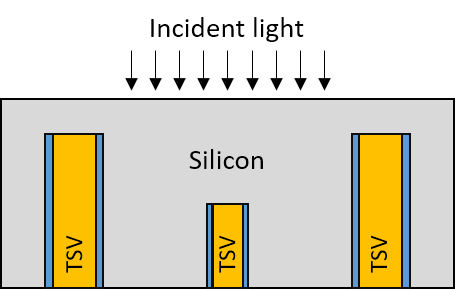
\includegraphics[width=2.5in]{figures/structure_general.png}
	\caption{	The general structure of a backside-connected TSV-based via collector solar cell.
				TSVs of varying size can be used to collect carriers at different depths within the cell without
			shadowing large portions of the silicon.}
	\label{f-via-collector-structure}
\end{figure}

For simplicity, we will first assume that the vias have zero diameter, and merely consider the effect of the
depth of the via termination from the silicon surface, $z_o$, the radius of the depletion region surrounding
the via termination, $r_d$, and the effective radius of collection, $r_c$. We are assuming both that the depletion
region is fully depleted, and that all photogenerated carriers within $r_c$ of the via termination are collected.
Additionally, we will initially ignore the impact of surface recombination, backside reflectors, antireflection coatings,
and vertical diffusion. These restrictions will gradually be relaxed as greater precision is required.
The simplified structure under consideration here is presented in \cref{f-via-collector-structure-simplified}.

\begin{figure}[tb]
	\centering
	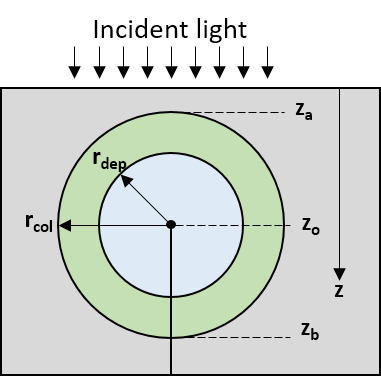
\includegraphics[width=2.5in]{figures/geometry_ideal.png}
	\caption{	The simplified structure under consideration for development of the compact model.
				For simplicity, TSVs are assumed to be infinitely thin, and all carriers generated within
				$r_{col}$ of the via termination are assumed to be collected.}
	\label{f-via-collector-structure-simplified}
\end{figure}
	

First, we must determine the carrier generation rate as a function of both wavelength and depth within the silicon.
We begin with the spectral irradiance, $I_R$, which has units of $W/m^2nm$, representing incident power density per
wavelength of illumination. Standard curves for AM0 (for space-based solar cells) and AM1.5 (for terrestrial solar cells)
can be found in the literature. We determine the spectral photon flux density at the device surface as
\begin{align}
	\phi_o(\lambda) &= I_R(\lambda)/E(\lambda)	\label{eq-spectral-flux-density}
\end{align}
where $E(\lambda)$ is the photon energy in Joules. The photon flux density at a depth $z$ within the silicon
is then given by
\begin{align}
	\phi(z) &= \phi_o e^{-\alpha z}	\label{eq-flux-density-depth}
\end{align}
where $\alpha$ is the (wavelength-dependent) absorption coefficient of silicon.

If we assume that every absorbed photon generates an electron-hole pair, the volumetric spectral carrier generation rate is
given by
\begin{align}
	g_{v\lambda}(z) &= -\frac{d\phi}{dz} \\
	g_{v\lambda}(z) &= \alpha \phi_o e^{-\alpha z}	\label{eq-generation-rate-depth}
\end{align}
We can now find the total (wavelength-dependent) carrier generation rate within a volume $dV$ by integrating
\begin{align}
	G_\lambda &= \int_{z_a}^{z_b} g_{v\lambda}(z) dV	\label{eq-generation-rate-integral-abstract}
\end{align}
In this case we are considering spherical collection regions with radius $r$, centered on a point at depth $z_o$.
Then $dV$ becomes $\pi p^2 dz$, where $p^2 = r^2 - (z-z_o)^2$ and \cref{eq-generation-rate-integral} becomes
\begin{align}
	G_\lambda &= \int_{z_a}^{z_b} \alpha \pi \phi_o \left(r^2- \left(z - z_o\right)^2\right) e^{-\alpha z} dz	\label{eq-generation-rate-integral}
\end{align}

Performing the integration, we arrive at a simple equation for the generation rate within our collection volume
\begin{align}
	G_\lambda = &\pi \alpha^{-2} \phi_o e^{-\alpha z_a} \left( G_{\lambda_A} + G_{\lambda_B} \right)	\label{eq-generation-rate-full}
\end{align}
\begin{align}
	G_{\lambda_A} &= e^{-\alpha z_a} \left( \alpha^2 (r^2-\Delta z_a^2 ) + 2\alpha\Delta z_a - 2\right)	\label{eq-generation-rate-full-A}	\\
	G_{\lambda_B} &= e^{-\alpha z_b} \left( \alpha^2 (r^2-\Delta z_b^2 ) + 2\alpha\Delta z_b + 2\right)	\label{eq-generation-rate-full-B}
\end{align}
where $\Delta z_a = z_o - z_a$ and $\Delta z_b = z_b - z_o$.

In the case where the sphere is fully enclosed in the silicon, and not clipped by the surface edges, \cref{eq-generation-rate-full-A,eq-generation-rate-full-B}
can be further simplified to
\begin{align}
	G_{\lambda_A} &= e^{-\alpha z_a} \left( 2\alpha r - 2\right)	\label{eq-generation-rate-simplified-A}	\\
	G_{\lambda_B} &= e^{-\alpha z_b} \left( 2\alpha r + 2\right)	\label{eq-generation-rate-simplified-B}
\end{align}

In order to find the total carrier generation rate in this volume, $G_\lambda$ must be integrated over the wavelength range of interest --
recall that $\alpha$ and $\phi_o$ are wavelength-dependent quantities. The total carrier generation rate in the collection sphere is
then given by
\begin{align}
	G(r) &= \int_{\lambda_a}^{\lambda_b} G_\lambda d\lambda
\end{align}

If we assume that no carriers can be generated in the depletion region, then we can find the total carrier generation $G_{sh}$ in the spherical
shell between $r_{dep}$ and $r_{col}$ by simply subtracting the generation rates of two appropriately-sized spheres
\begin{align}
	G_{sh} &= G(r_{col}) - G(r_{dep})	\label{eq-generation-rate-shell}
\end{align}

\subsection{Estimating Collection Efficiency}
The strength of the via-based collection scheme is that carriers can be collected at a range of different heights
throughout the silicon, in order to capture carriers generated by a greater range of wavelengths. We will initially consider collection
volumes stacked in an FCC pattern, as shown in \cref{f-collection-volume-stack}. In this configuration, each collection volume
is vertically separated from its nearest vertical neighbors by a depth of $\sqrt{3}r$. Since each collection volume is placed
to avoid overlap, we can simply sum up the contributions of each volume to determine the total carrier collection rate.
\begin{align}
	G_{tot} &= \sum_n G_{sh}(z=z_o + nr\sqrt{3})	\label{eq-generation-rate-unit-cell}
\end{align}

\begin{figure}[tb]
	\centering
	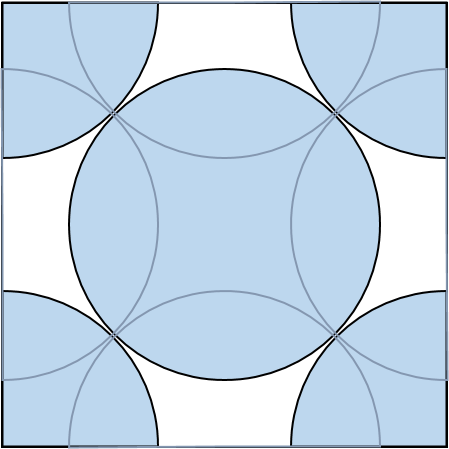
\includegraphics[width=2.0in]{figures/fcc_top_view.png}
	\caption{	Top view of the FCC collection sphere placement unit cell. Upper spheres have black borders,
				and lower spheres have blue borders.}
	\label{f-collection-volume-stack}
\end{figure}

The overall carrier collection efficiency can then be calculated as
\begin{align}
	\eta_{col} &= \frac{G_{tot} / A_{uc} }{\Phi}	\label{eq-collection-efficiency}
\end{align}
where $A_{uc} = 4r^2$ is the area of the unit cell and $\Phi$ is the total photon flux density, given by
\begin{align}
	\Phi &= \int_{\lambda_a}^{\lambda_b} \phi_o(\lambda)
\end{align}

\section{Preliminary Results}
Using \cref{eq-generation-rate-unit-cell,eq-collection-efficiency}, we can determine the collection efficiency
for a range of interesting structures. For instance, we can consider a case where we can stack arbitrary numbers
of collection volumes on top of one another, in which case we should expect the overall collection efficiency
to increase with the number of collection tiers. The collection efficiency for this case, assuming illumination with the AM0
spectra, and with $r_{dep}=1\mu m$ and $r_{col} = 4\mu m$ is shown in
\cref{f-collection-efficiency-arbitrary-tiers}.

\begin{figure}[tb]
	\centering
	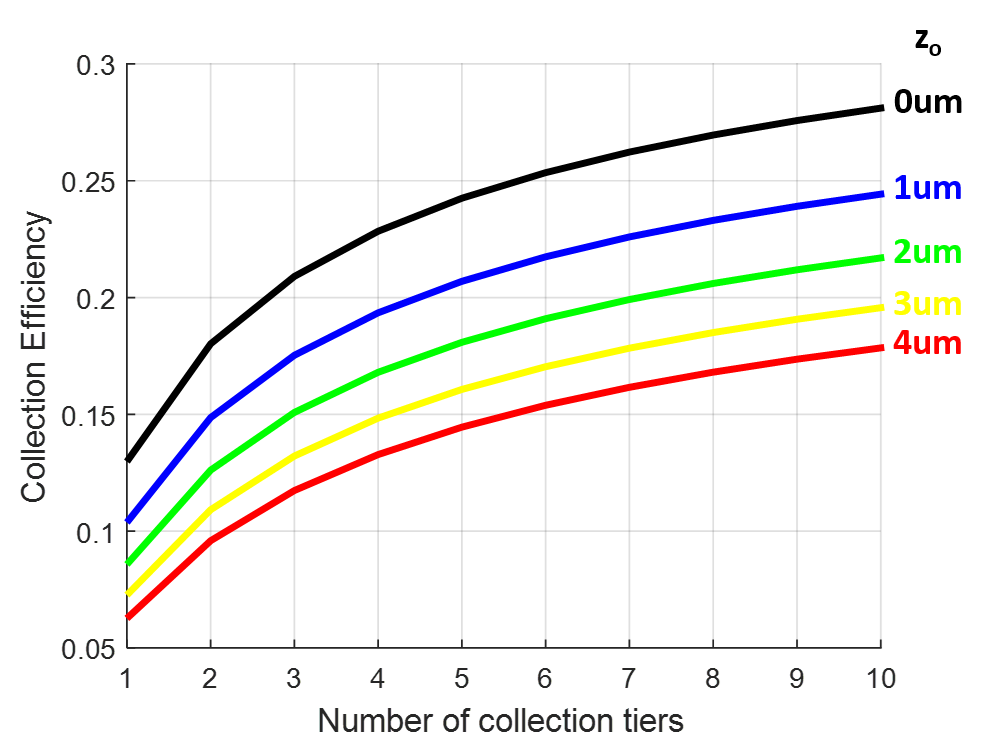
\includegraphics[width=3.5in]{figures/eta_col_fcc_stack_arbitrary_tiers.png}
	\caption{	The collection efficiency in the case where an arbitrary number of collection tiers can be stacked.
				The collection efficiency varies significantly with $z_o$, the depth of the top collection tier.
			}
	\label{f-collection-efficiency-arbitrary-tiers}
\end{figure}


\end{document}
